\documentclass{article}
\usepackage[T1]{tipa}
\usepackage{dirtytalk}
\usepackage{listings}
\usepackage{graphicx}
\graphicspath{ {imagenes/} }
\usepackage{wrapfig}
\usepackage{multicol}
\usepackage{fancyhdr}
\usepackage{hyperref}

%----------------------------------------------------------------------------------------
% PAGE STYLE
%----------------------------------------------------------------------------------------

\topmargin=-0.45in
\evensidemargin=0in
\oddsidemargin=0in
\textwidth=6.5in
\textheight=9.0in
\headsep=0.25in

\linespread{1.1}

\pagestyle{fancy}

%----------------------------------------------------------------------------------------
%	ASSIGNMENT INFORMATION
%----------------------------------------------------------------------------------------

\title{Matem\'{a}ticas Discr\'{e}tas: Reporte \#1} % Title of the assignment
\author{Diego Navarro}
\date{UNAM, Facultad de Ciencias --- \today}

%----------------------------------------------------------------------------------------

\begin{document}

\maketitle
\pagebreak

%----------------------------------------------------------------------------------------
%	INTRODUCTION
%----------------------------------------------------------------------------------------

\section*{Alan Turing}
\begin{wrapfigure}{r}{0.35\textwidth}
  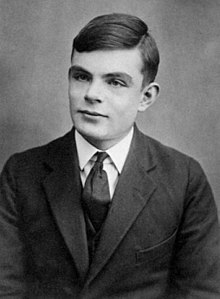
\includegraphics[width=0.35\textwidth]{turing}
\end{wrapfigure}
\textbf{Alan Mathison Turing} OBE FRS (\textipa{/"tjU@rIN/}; 23 June 1912 – 7 June 1954) was an English mathematician, computer scientist, logician, cryptanalyst, philosopher, and theoretical biologist. Turing was highly influential in the development of theoretical computer science, providing a formalisation of the concepts of algorithm and computation with the Turing machine, which can be considered a model of a general-purpose computer. Turing is widely considered to be the father of theoretical computer science and artificial intelligence. Despite these accomplishments, he was never fully recognised in his home country during his lifetime due to the prevalence of homophobia at the time and because much of his work was covered by the Official Secrets Act.\\
\\
During the Second World War, Turing worked for the Government Code and Cypher School (GC\&CS) at Bletchley Park, Britain's codebreaking centre that produced Ultra intelligence. For a time he led Hut 8, the section that was responsible for German naval cryptanalysis. Here, he devised a number of techniques for speeding the breaking of German ciphers, including improvements to the pre-war Polish bombe method, an electromechanical machine that could find settings for the Enigma machine.\\
\\
Turing played a crucial role in cracking intercepted coded messages that enabled the Allies to defeat the Nazis in many crucial engagements, including the Battle of the Atlantic, and in so doing helped win the war. Due to the problems of counterfactual history, it is hard to estimate the precise effect Ultra intelligence had on the war, but at the upper end it has been estimated that this work shortened the war in Europe by more than two years and saved over 14 million lives.\\
\\
After the war Turing worked at the National Physical Laboratory, where he designed the Automatic Computing Engine. The Automatic Computing Engine was one of the first designs for a stored-program computer. In 1948, Turing joined Max Newman's Computing Machine Laboratory, at the Victoria University of Manchester, where he helped develop the Manchester computers and became interested in mathematical biology. He wrote a paper on the chemical basis of morphogenesis and predicted oscillating chemical reactions such as the Belousov–Zhabotinsky reaction, first observed in the 1960s.\\
\\
Turing was prosecuted in 1952 for homosexual acts; the Labouchere Amendment of 1885 had mandated that "gross indecency" was a criminal offence in the UK. He accepted chemical castration treatment, with DES, as an alternative to prison. Turing died in 1954, 16 days before his 42nd birthday, from cyanide poisoning. An inquest determined his death as a suicide, but it has been noted that the known evidence is also consistent with accidental poisoning.\\
\\
In 2009, following an Internet campaign, British Prime Minister Gordon Brown made an official public apology on behalf of the British government for "the appalling way he was treated". Queen Elizabeth II granted Turing a posthumous pardon in 2013. The "Alan Turing law" is now an informal term for a 2017 law in the United Kingdom that retroactively pardoned men cautioned or convicted under historical legislation that outlawed homosexual acts.\\

\section{Career and research}

When Turing returned to Cambridge, he attended lectures given in 1939 by Ludwig Wittgenstein about the foundations of mathematics. The lectures have been reconstructed verbatim, including interjections from Turing and other students, from students' notes. Turing and Wittgenstein argued and disagreed, with Turing defending formalism and Wittgenstein propounding his view that mathematics does not discover any absolute truths, but rather invents them.\\

\subsection{Cryptanalysis}

During the Second World War, Turing was a leading participant in the breaking of German ciphers at Bletchley Park. The historian and wartime codebreaker Asa Briggs has said, "You needed exceptional talent, you needed genius at Bletchley and Turing's was that genius."\\
From September 1938, Turing worked part-time with the Government Code and Cypher School (GC\&CS), the British codebreaking organisation. He concentrated on cryptanalysis of the Enigma cipher machine used by Nazi Germany, together with Dilly Knox, a senior GC\&CS codebreaker. Soon after the July 1939 meeting near Warsaw at which the Polish Cipher Bureau gave the British and French details of the wiring of Enigma machine's rotors and their method of decrypting Enigma machine's messages, Turing and Knox developed a broader solution. The Polish method relied on an insecure indicator procedure that the Germans were likely to change, which they in fact did in May 1940. Turing's approach was more general, using crib-based decryption for which he produced the functional specification of the bombe (an improvement on the Polish Bomba).\\
Two cottages in the stable yard at Bletchley Park. Turing worked here in 1939 and 1940, before moving to Hut 8.\\
\\
On 4 September 1939, the day after the UK declared war on Germany, Turing reported to Bletchley Park, the wartime station of GC\&CS. Specifying the bombe was the first of five major cryptanalytical advances that Turing made during the war. The others were: deducing the indicator procedure used by the German navy; developing a statistical procedure dubbed Banburismus for making much more efficient use of the bombes; developing a procedure dubbed Turingery for working out the cam settings of the wheels of the Lorenz SZ 40/42 (Tunny) cipher machine and, towards the end of the war, the development of a portable secure voice scrambler at Hanslope Park that was codenamed Delilah.\\
\\
By using statistical techniques to optimise the trial of different possibilities in the code breaking process, Turing made an innovative contribution to the subject. He wrote two papers discussing mathematical approaches, titled The Applications of Probability to Cryptography and Paper on Statistics of Repetitions, which were of such value to GC\&CS and its successor GCHQ that they were not released to the UK National Archives until April 2012, shortly before the centenary of his birth. A GCHQ mathematician, "who identified himself only as Richard," said at the time that the fact that the contents had been restricted for some 70 years demonstrated their importance, and their relevance to post-war cryptanalysis:\\
\\
    \say{[He] said the fact that the contents had been restricted "shows what a tremendous importance it has in the foundations of our subject". ... The papers detailed using "mathematical analysis to try and determine which are the more likely settings so that they can be tried as quickly as possible." ... Richard said that GCHQ had now "squeezed the juice" out of the two papers and was "happy for them to be released into the public domain".}
\\\\
Turing had a reputation for eccentricity at Bletchley Park. He was known to his colleagues as "Prof" and his treatise on Enigma was known as the "Prof's Book". According to historian Ronald Lewin, Jack Good, a cryptanalyst who worked with Turing, said of his colleague:
\\\\
    \say{In the first week of June each year he would get a bad attack of hay fever, and he would cycle to the office wearing a service gas mask to keep the pollen off. His bicycle had a fault: the chain would come off at regular intervals. Instead of having it mended he would count the number of times the pedals went round and would get off the bicycle in time to adjust the chain by hand. Another of his eccentricities is that he chained his mug to the radiator pipes to prevent it being stolen.}
\\\\
Peter Hilton recounted his experience working with Turing in Hut 8 in his "Reminiscences of Bletchley Park" from A Century of Mathematics in America:
\\\\
    \say{It is a rare experience to meet an authentic genius. Those of us privileged to inhabit the world of scholarship are familiar with the intellectual stimulation furnished by talented colleagues. We can admire the ideas they share with us and are usually able to understand their source; we may even often believe that we ourselves could have created such concepts and originated such thoughts. However, the experience of sharing the intellectual life of a genius is entirely different; one realizes that one is in the presence of an intelligence, a sensibility of such profundity and originality that one is filled with wonder and excitement. Alan Turing was such a genius, and those, like myself, who had the astonishing and unexpected opportunity, created by the strange exigencies of the Second World War, to be able to count Turing as colleague and friend will never forget that experience, nor can we ever lose its immense benefit to us.}
\\\\
Hilton echoed similar thoughts in the Nova PBS documentary Decoding Nazi Secrets.
\\\\
While working at Bletchley, Turing, who was a talented long-distance runner, occasionally ran the 40 miles (64 km) to London when he was needed for meetings, and he was capable of world-class marathon standards. Turing tried out for the 1948 British Olympic team but he was hampered by an injury. His tryout time for the marathon was only 11 minutes slower than British silver medallist Thomas Richards' Olympic race time of 2 hours 35 minutes. He was Walton Athletic Club's best runner, a fact discovered when he passed the group while running alone.
\\\\
In 1946, Turing was appointed an Officer of the Order of the British Empire (OBE) by King George VI for his wartime services, but his work remained secret for many years.

\subsection{Bombe}

Within weeks of arriving at Bletchley Park, Turing had specified an electromechanical machine called the bombe, which could break Enigma more effectively than the Polish bomba kryptologiczna, from which its name was derived. The bombe, with an enhancement suggested by mathematician Gordon Welchman, became one of the primary tools, and the major automated one, used to attack Enigma-enciphered messages.
\\\\
A complete and working replica of a bombe now at The National Museum of Computing on Bletchley Park
\\\\
The bombe searched for possible correct settings used for an Enigma message (i.e., rotor order, rotor settings and plugboard settings) using a suitable crib: a fragment of probable plaintext. For each possible setting of the rotors (which had on the order of 1019 states, or 1022 states for the four-rotor U-boat variant), the bombe performed a chain of logical deductions based on the crib, implemented electromechanically.
\\\\
The bombe detected when a contradiction had occurred and ruled out that setting, moving on to the next. Most of the possible settings would cause contradictions and be discarded, leaving only a few to be investigated in detail. A contradiction would occur when an enciphered letter would be turned back into the same plaintext letter, which was impossible with the Enigma. The first bombe was installed on 18 March 1940.
\\\\
By late 1941, Turing and his fellow cryptanalysts Gordon Welchman, Hugh Alexander and Stuart Milner-Barry were frustrated. Building on the work of the Poles, they had set up a good working system for decrypting Enigma signals, but their limited staff and bombes meant they could not translate all the signals. In the summer, they had considerable success, and shipping losses had fallen to under 100,000 tons a month; however, they badly needed more resources to keep abreast of German adjustments. They had tried to get more people and fund more bombes through the proper channels, but had failed.
\\\\
On 28 October they wrote directly to Winston Churchill explaining their difficulties, with Turing as the first named. They emphasised how small their need was compared with the vast expenditure of men and money by the forces and compared with the level of assistance they could offer to the forces. As Andrew Hodges, biographer of Turing, later wrote, "This letter had an electric effect." Churchill wrote a memo to General Ismay, which read: "ACTION THIS DAY. Make sure they have all they want on extreme priority and report to me that this has been done." On 18 November, the chief of the secret service reported that every possible measure was being taken. The cryptographers at Bletchley Park did not know of the Prime Minister's response, but as Milner-Barry recalled, "All that we did notice was that almost from that day the rough ways began miraculously to be made smooth." More than two hundred bombes were in operation by the end of the war.
\\\\
Statue of Turing by Stephen Kettle at Bletchley Park, commissioned by Sidney Frank, built from half a million pieces of Welsh slate.
\\\\
\subsection{Hut 8 and the naval Enigma}

\begin{figure}
  \centering
  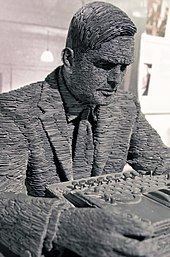
\includegraphics[width=0.25\textwidth]{turing_statue}
\end{figure}

Turing decided to tackle the particularly difficult problem of German naval Enigma "because no one else was doing anything about it and I could have it to myself". In December 1939, Turing solved the essential part of the naval indicator system, which was more complex than the indicator systems used by the other services.
\\\\
That same night, he also conceived of the idea of Banburismus, a sequential statistical technique (what Abraham Wald later called sequential analysis) to assist in breaking the naval Enigma, "though I was not sure that it would work in practice, and was not, in fact, sure until some days had actually broken." For this, he invented a measure of weight of evidence that he called the ban. Banburismus could rule out certain sequences of the Enigma rotors, substantially reducing the time needed to test settings on the bombes. Later this sequential process of accumulating sufficient weight of evidence using decibans (one tenth of a ban) was used in Cryptanalysis of the Lorenz cipher.
\\\\
Turing travelled to the United States in November 1942 and worked with US Navy cryptanalysts on the naval Enigma and bombe construction in Washington; he also visited their Computing Machine Laboratory in Dayton, Ohio.
\\\\
Turing's reaction to the American bombe design was far from enthusiastic:
\\\\
    \say{The American Bombe programme was to produce 336 Bombes, one for each wheel order. I used to smile inwardly at the conception of Bombe hut routine implied by this programme, but thought that no particular purpose would be served by pointing out that we would not really use them in that way. Their test (of commutators) can hardly be considered conclusive as they were not testing for the bounce with electronic stop finding devices. Nobody seems to be told about rods or offiziers or banburismus unless they are really going to do something about it.}
\\\\
During this trip, he also assisted at Bell Labs with the development of secure speech devices. He returned to Bletchley Park in March 1943. During his absence, Hugh Alexander had officially assumed the position of head of Hut 8, although Alexander had been de facto head for some time (Turing having little interest in the day-to-day running of the section). Turing became a general consultant for cryptanalysis at Bletchley Park.
\\\\
Alexander wrote of Turing's contribution:
\\\\
    \say{There should be no question in anyone's mind that Turing's work was the biggest factor in Hut 8's success. In the early days, he was the only cryptographer who thought the problem worth tackling and not only was he primarily responsible for the main theoretical work within the Hut, but he also shared with Welchman and Keen the chief credit for the invention of the bombe. It is always difficult to say that anyone is 'absolutely indispensable', but if anyone was indispensable to Hut 8, it was Turing. The pioneer's work always tends to be forgotten when experience and routine later make everything seem easy and many of us in Hut 8 felt that the magnitude of Turing's contribution was never fully realised by the outside world.}

\subsection{Turingery}

In July 1942, Turing devised a technique termed Turingery (or jokingly Turingismus) for use against the Lorenz cipher messages produced by the Germans' new Geheimschreiber (secret writer) machine. This was a teleprinter rotor cipher attachment codenamed Tunny at Bletchley Park. Turingery was a method of wheel-breaking, i.e., a procedure for working out the cam settings of Tunny's wheels. He also introduced the Tunny team to Tommy Flowers who, under the guidance of Max Newman, went on to build the Colossus computer, the world's first programmable digital electronic computer, which replaced a simpler prior machine (the Heath Robinson), and whose superior speed allowed the statistical decryption techniques to be applied usefully to the messages. Some have mistakenly said that Turing was a key figure in the design of the Colossus computer. Turingery and the statistical approach of Banburismus undoubtedly fed into the thinking about cryptanalysis of the Lorenz cipher, but he was not directly involved in the Colossus development.

\subsection{Delilah}

Following his work at Bell Labs in the US, Turing pursued the idea of electronic enciphering of speech in the telephone system. In the latter part of the war, he moved to work for the Secret Service's Radio Security Service (later HMGCC) at Hanslope Park. At the park, he further developed his knowledge of electronics with the assistance of engineer Donald Bayley. Together they undertook the design and construction of a portable secure voice communications machine codenamed Delilah. The machine was intended for different applications, but it lacked the capability for use with long-distance radio transmissions. In any case, Delilah was completed too late to be used during the war. Though the system worked fully, with Turing demonstrating it to officials by encrypting and decrypting a recording of a Winston Churchill speech, Delilah was not adopted for use. Turing also consulted with Bell Labs on the development of SIGSALY, a secure voice system that was used in the later years of the war.
\\\\
\subsection{Early computers and the Turing test}
Plaque, 78 High Street, Hampton
\\\\
Between 1945 and 1947, Turing lived in Hampton, London, while he worked on the design of the ACE (Automatic Computing Engine) at the National Physical Laboratory (NPL). He presented a paper on 19 February 1946, which was the first detailed design of a stored-program computer. Von Neumann's incomplete First Draft of a Report on the EDVAC had predated Turing's paper, but it was much less detailed and, according to John R. Womersley, Superintendent of the NPL Mathematics Division, it "contains a number of ideas which are Dr. Turing's own". Although ACE was a feasible design, the secrecy surrounding the wartime work at Bletchley Park led to delays in starting the project and he became disillusioned. In late 1947 he returned to Cambridge for a sabbatical year during which he produced a seminal work on Intelligent Machinery that was not published in his lifetime. While he was at Cambridge, the Pilot ACE was being built in his absence. It executed its first program on 10 May 1950, and a number of later computers around the world owe much to it, including the English Electric DEUCE and the American Bendix G-15. The full version of Turing's ACE was not built until after his death.
\\\\
According to the memoirs of the German computer pioneer Heinz Billing from the Max Planck Institute for Physics, published by Genscher, Düsseldorf, there was a meeting between Turing and Konrad Zuse. It took place in Göttingen in 1947. The interrogation had the form of a colloquium. Participants were Womersley, Turing, Porter from England and a few German researchers like Zuse, Walther, and Billing (for more details see Herbert Bruderer, Konrad Zuse und die Schweiz).
\\\\
In 1948, Turing was appointed reader in the Mathematics Department at the Victoria University of Manchester. A year later, he became Deputy Director of the Computing Machine Laboratory, where he worked on software for one of the earliest stored-program computers—the Manchester Mark 1. Turing wrote the first version of the Programmer's Manual for this machine, and was recruited by Ferranti as a consultant in the development of their commercialised machine, the Ferranti Mark 1. He continued to be paid consultancy fees by Ferranti until his death. During this time, he continued to do more abstract work in mathematics, and in "Computing Machinery and Intelligence" (Mind, October 1950), Turing addressed the problem of artificial intelligence, and proposed an experiment that became known as the Turing test, an attempt to define a standard for a machine to be called "intelligent". The idea was that a computer could be said to "think" if a human interrogator could not tell it apart, through conversation, from a human being. In the paper, Turing suggested that rather than building a program to simulate the adult mind, it would be better to produce a simpler one to simulate a child's mind and then to subject it to a course of education. A reversed form of the Turing test is widely used on the Internet; the CAPTCHA test is intended to determine whether the user is a human or a computer.
\\\\
In 1948 Turing, working with his former undergraduate colleague, D.G. Champernowne, began writing a chess program for a computer that did not yet exist. By 1950, the program was completed and dubbed the Turochamp. In 1952, he tried to implement it on a Ferranti Mark 1, but lacking enough power, the computer was unable to execute the program. Instead, Turing "ran" the program by flipping through the pages of the algorithm and carrying out its instructions on a chessboard, taking about half an hour per move. The game was recorded. According to Garry Kasparov, Turing's program "played a recognizable game of chess." The program lost to Turing's colleague Alick Glennie, although it is said that it won a game against Champernowne's wife, Isabel.
\\\\
His Turing test was a significant, characteristically provocative, and lasting contribution to the debate regarding artificial intelligence, which continues after more than half a century.
\\\\
Pattern formation and mathematical biology
\\\\
When Turing was 39 years old in 1951, he turned to mathematical biology, finally publishing his masterpiece "The Chemical Basis of Morphogenesis" in January 1952. He was interested in morphogenesis, the development of patterns and shapes in biological organisms. He suggested that a system of chemicals reacting with each other and diffusing across space, termed a reaction-diffusion system, could account for "the main phenomena of morphogenesis". He used systems of partial differential equations to model catalytic chemical reactions. For example, if a catalyst A is required for a certain chemical reaction to take place, and if the reaction produced more of the catalyst A, then we say that the reaction is autocatalytic, and there is positive feedback that can be modelled by nonlinear differential equations. Turing discovered that patterns could be created if the chemical reaction not only produced catalyst A, but also produced an inhibitor B that slowed down the production of A. If A and B then diffused through the container at different rates, then you could have some regions where A dominated and some where B did. To calculate the extent of this, Turing would have needed a powerful computer, but these were not so freely available in 1951, so he had to use linear approximations to solve the equations by hand. These calculations gave the right qualitative results, and produced, for example, a uniform mixture that oddly enough had regularly spaced fixed red spots. The Russian biochemist Boris Belousov had performed experiments with similar results, but could not get his papers published because of the contemporary prejudice that any such thing violated the second law of thermodynamics. Belousov was not aware of Turing's paper in the Philosophical Transactions of the Royal Society.
\\\\
Although published before the structure and role of DNA was understood, Turing's work on morphogenesis remains relevant today and is considered a seminal piece of work in mathematical biology. One of the early applications of Turing's paper was the work by James Murray explaining spots and stripes on the fur of cats, large and small. Further research in the area suggests that Turing's work can partially explain the growth of "feathers, hair follicles, the branching pattern of lungs, and even the left-right asymmetry that puts the heart on the left side of the chest." In 2012, Sheth, et al. found that in mice, removal of Hox genes causes an increase in the number of digits without an increase in the overall size of the limb, suggesting that Hox genes control digit formation by tuning the wavelength of a Turing-type mechanism. Later papers were not available until Collected Works of A. M. Turing was published in 1992.

\section{Otras cosas faltantes}
  \subsection{Cr\'editos:}
    Todo lo anterior fue sacado de \href{https://en.wikipedia.org/wiki/Alan\_Turing}{Wikipedia}, de
    la secci\'on 2 \href{https://en.wikipedia.org/wiki/Alan\_Turing#Career\_and\_research}{Career and reaserch}.
  \subsection{Tablas:}
    \begin{tabular}{c || c |c | c |c}
      \textbf{1} & \textbf{8} & \textbf{9} & \textbf{h} & \textbf{i} \\ \hline \hline
      2 & 7 & a & g & j \\ \hline
      3 & 6 & b & f & k \\ \hline
      4 & 5 & c & d & l
    \end{tabular}
  \subsection{Code:}

    \begin{lstlisting}
import numpy as np

def incmatrix(genl1,genl2):
    m = len(genl1)
    n = len(genl2)
    M = None #to become the incidence matrix
    VT = np.zeros((n*m,1), int)  #dummy variable

    #compute the bitwise xor matrix
    M1 = bitxormatrix(genl1)
    M2 = np.triu(bitxormatrix(genl2),1)

    for i in range(m-1):
        for j in range(i+1, m):
            [r,c] = np.where(M2 == M1[i,j])
            for k in range(len(r)):
                VT[(i)*n + r[k]] = 1;
                VT[(i)*n + c[k]] = 1;
                VT[(j)*n + r[k]] = 1;
                VT[(j)*n + c[k]] = 1;

                if M is None:
                    M = np.copy(VT)
                else:
                    M = np.concatenate((M, VT), 1)

                VT = np.zeros((n*m,1), int)

    return M
    \end{lstlisting}

  \subsection{Lists:}
    \begin{itemize}
      \item{First}
      \item{Second}
      \item{third}
    \end{itemize}
    \begin{enumerate}
      \item The labels consists of sequential numbers.
      \item The numbers starts at 1 with every call to the enumerate environment.
    \end{enumerate}
  \subsection{Imagen en hoja sola:}
    \pagebreak

    \begin{figure}
      Turing's OBE currently held in Sherborne School archives
      \centering
      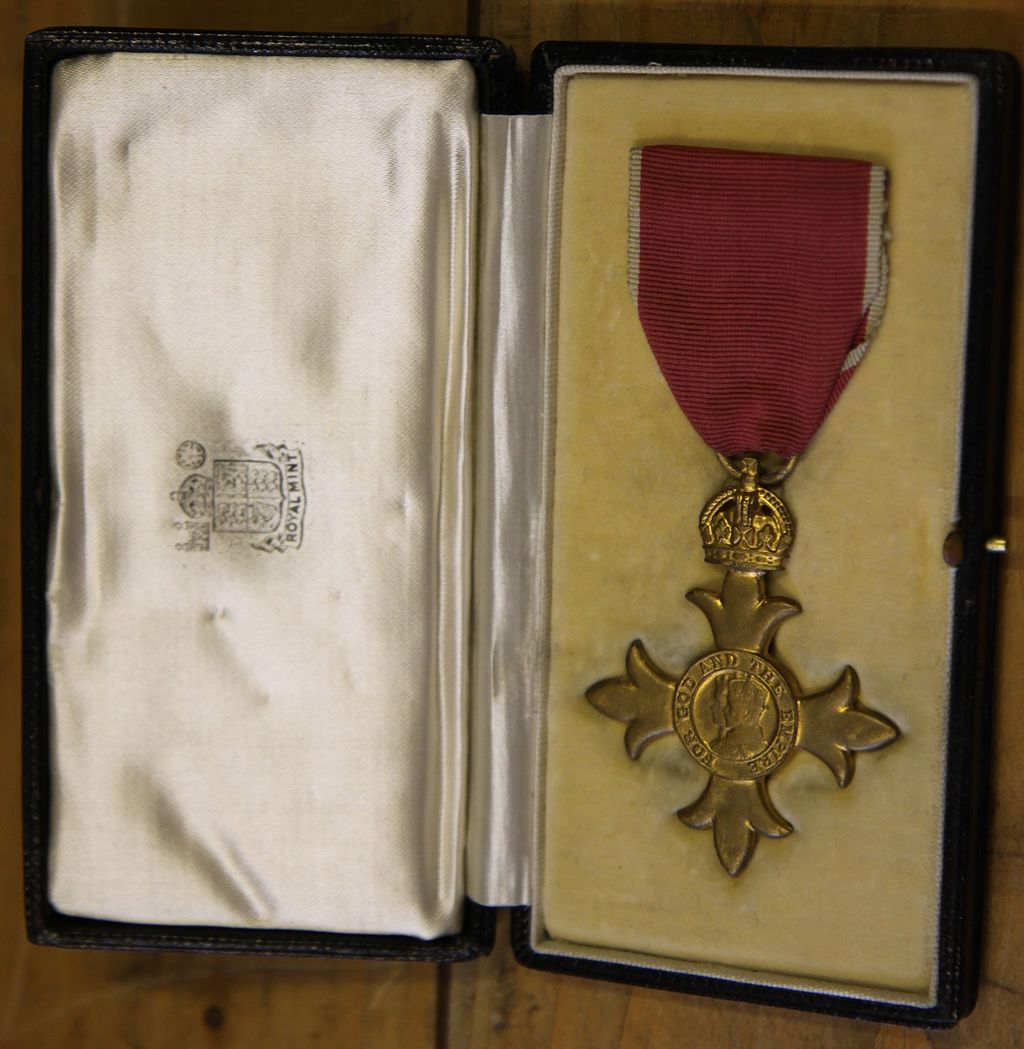
\includegraphics[width=0.85\textwidth]{OBE}
    \end{figure}
\end{document}
